\section{Experiments}
\label{sec:experiments}

We evaluate SAVNav on the benchmark introduced in Section~\ref{sec:benchmark} from three complementary perspectives. First, we test whether a single system can simultaneously satisfy the coupled requirements of acoustic target reaching, human safety, and social compliance. Second, we test whether the gains come from persistent structured reasoning in SAVMap rather than from richer multi-modal sensing alone. Third, we isolate which capabilities in SAVMap and the SAVNav policy are responsible for performance in LOS social routing, NLOS acoustic anticipation, and ambiguity-aware target search.

\subsection{Experimental Setup}
\label{subsec:exp-setup}

We conduct all simulation experiments in Habitat 3.0 with SoundSpaces 2.0 acoustic rendering, using the benchmark protocol from Section~\ref{sec:benchmark}. The three scenarios stress different aspects of the SAVNav task. Crowded Social evaluates LOS social routing around visible SCGs and DPs, Hidden Boundary isolates NLOS acoustic anticipation at blind corners, and Mixed Home Activity evaluates whether a policy can jointly handle target search, visible social boundaries, and acoustically inferred NLOS risks in the same episode. Unless otherwise noted, all compared methods share the same episode budget ($T_{max}=500$), success criterion ($d_{success}=1.0\,\mathrm{m}$), and evaluation metrics.

To rigorously isolate the contribution of each system component, we design our baselines and ablations as orthogonal functional degradations along three dimensions: memory, space, and search. Rather than treating missing components as simple on-off switches (which would lead to trivial failure modes, such as treating humans as geometric obstacles), we replace our advanced mechanisms with naive or greedy algorithmic alternatives. This strictly controls variables and isolates the specific value of structured reasoning.

We compare SAVNav against three baselines chosen to expose distinct failure modes of the SAVNav task. Falcon+Goal Oracle represents strong LOS social navigation without acoustic social reasoning; ENMuS\textsuperscript{3} represents target-seeking audio-visual navigation without social boundary modeling; and Reactive SAVNav shares the same perception front-end as our full system but removes persistent map-level reasoning. These baselines are adapted only as needed to make them operational on our benchmark, and each is evaluated in the strongest setting consistent with its original design assumptions.

\begin{enumerate}
	\item \textit{Falcon+Goal Oracle:} Falcon~\cite{CognitionPrecognitionFutureaware2025} is a vision-based social navigation method that predicts human motion from egocentric observations. Because it is not designed for acoustic target search, we provide the ground-truth target location as a navigation goal oracle while keeping all human reasoning purely vision-based. This adaptation isolates the limitation of LOS-only social reasoning: Falcon can react to visible humans, but it cannot use \texttt{conversation} or \texttt{footsteps} as NLOS social cues.
	\item \textit{ENMuS\textsuperscript{3}:} ENMuS\textsuperscript{3}~\cite{AudiovisualNavigationNoisy2025} is a multi-source audio-visual navigation framework for category-conditioned sound seeking. We map our query tokens to aligned BeDAViN target categories when available (\texttt{doorbell}, \texttt{television}, and \texttt{water tap}). Episodes with the \texttt{human call} target are excluded for this baseline because ENMuS\textsuperscript{3} has no semantically aligned target category. ENMuS\textsuperscript{3} therefore serves as a socially-unaware AVNav baseline: it uses audio to pursue the acoustic target but does not interpret human-generated sounds as social boundaries.
	\item \textit{Reactive SAVNav:} This baseline ablates the memory dimension by removing all inter-frame accumulation ($\lambda=0$ in topological anticipation, and $S_{anch}^{(t-1)}=0$ in anchoring). It shares our multi-modal perception front-end but retains no persistent states: no audio-visual anchoring memory, no target spatial belief map $\mathcal{B}(\mathbf{x})$, and no node probability accumulation. At each frame, acoustic events are greedily matched against all entities. If the acoustic target remains unanchored, the system cannot compute information gain $U(\mathbf{p}_i)$; instead, it falls back to a greedy search strategy, projecting a waypoint at a fixed look-ahead distance $r_{react}$ along the current target DOA $\mathbf{d}_{world}$. This tests whether instantaneous multi-modal reactions are sufficient without persistent spatio-temporal memory.
\end{enumerate}

\subsection{Main Results in Simulation}
\label{subsec:exp-main}

Table~\ref{tab:main_results} reports the quantitative performance of SAVNav and the baselines across the three scenarios.

\begin{table*}[t]
	\centering
	\caption{Main results on the SAVNav benchmark. ENMuS\textsuperscript{3} is evaluated only on episodes whose target categories admit aligned BeDAViN mappings. NCR in Crowded Social is marked as `--' because that scenario contains no NLOS human risk by definition.}
	\label{tab:main_results}
	\resizebox{\linewidth}{!}{
		\begin{tabular}{l | ccccc | ccccc | ccccc}
			\toprule
			\multirow{2}{*}{Method}  & \multicolumn{5}{c|}{Crowded Social} & \multicolumn{5}{c|}{Hidden Boundary} & \multicolumn{5}{c}{Mixed Home Activity}                                     \\
			\cmidrule(lr){2-6} \cmidrule(lr){7-11} \cmidrule(lr){12-16}
			                         & SR $\uparrow$                       & SPL $\uparrow$                       & HCR $\downarrow$                        & NCR $\downarrow$ & PSC $\uparrow$
			                         & SR $\uparrow$                       & SPL $\uparrow$                       & HCR $\downarrow$                        & NCR $\downarrow$ & PSC $\uparrow$
			                         & SR $\uparrow$                       & SPL $\uparrow$                       & HCR $\downarrow$                        & NCR $\downarrow$ & PSC $\uparrow$ \\
			\midrule
			Falcon+Goal Oracle       & \textbf{55.12}                      & \textbf{50.38}                       & 35.67                                   & --               & 87.24
			                         & 36.25                               & 32.17                                & 56.48                                   & 48.73            & 82.35
			                         & 40.18                               & 35.42                                & 50.36                                   & 36.24            & 83.47          \\
			ENMuS\textsuperscript{3} & 25.83                               & 16.47                                & 42.15                                   & --               & 66.38
			                         & 30.42                               & 19.86                                & 46.53                                   & 39.27            & 71.84
			                         & 21.36                               & 13.28                                & 50.83                                   & 30.52            & 64.53          \\
			Reactive SAVNav          & 42.56                               & 31.74                                & 23.41                                   & --               & 82.63
			                         & 36.83                               & 27.54                                & 36.12                                   & 29.47            & 79.62
			                         & 36.45                               & 27.13                                & 29.84                                   & 22.36            & 80.28          \\
			\midrule
			SAVNav (Ours)            & 54.28                               & 43.15                                & \textbf{13.52}                          & --               & \textbf{90.17}
			                         & \textbf{51.47}                      & \textbf{41.23}                       & \textbf{17.85}                          & \textbf{11.36}   & \textbf{88.74}
			                         & \textbf{49.52}                      & \textbf{39.47}                       & \textbf{15.63}                          & \textbf{9.84}    & \textbf{88.36} \\
			\bottomrule
		\end{tabular}
	}
\end{table*}

Compared with Falcon+Goal Oracle, SAVNav is most clearly differentiated in scenarios where social reasoning must extend beyond LOS observations. In Hidden Boundary, SAVNav improves SR from 36.25 to 51.47 and SPL from 32.17 to 41.23, while reducing HCR from 56.48 to 17.85 and NCR from 48.73 to 11.36. This gap is not a generic navigation gain; it directly reflects the value of topology-aware acoustic anticipation, because Falcon can only respond after the human becomes visible. The same pattern persists in Mixed Home Activity, where SAVNav improves SR by 9.34 points and reduces NCR by 26.40 points, showing that the policy can jointly handle visible humans, NLOS risks, and target pursuit.

Compared with ENMuS\textsuperscript{3}, SAVNav exposes the limitations of socially-unaware target seeking. ENMuS\textsuperscript{3} can follow target-related sound cues, but it does not convert \texttt{conversation} or \texttt{footsteps} into planner-relevant social boundaries. The result is a severe degradation in both safety and compliance. In Crowded Social, SAVNav improves PSC from 66.38 to 90.17 and reduces HCR from 42.15 to 13.52. In Mixed Home Activity, the same gap remains pronounced, with SAVNav improving SR by 28.16 points and reducing HCR by 35.20 points. These results show that acoustic target navigation alone is insufficient for the SAVNav task.

The comparison with Reactive SAVNav isolates the effect of persistent structured reasoning, because both methods share the same perception front-end. Across all scenarios, SAVNav consistently improves both efficiency and safety over the reactive variant. The difference is especially strong in Hidden Boundary, where SAVNav reduces NCR from 29.47 to 11.36 and improves SPL from 27.54 to 41.23, indicating that stable NLOS yielding requires persistent node-level risk accumulation rather than frame-by-frame reaction. In Mixed Home Activity, SAVNav also improves SR from 36.45 to 49.52, confirming that target reasoning and social reasoning must coexist at the map level rather than being recomputed greedily at each step.

\subsection{Ablation Study}
\label{subsec:exp-ablation}

To isolate the contribution of each capability, we evaluate three ablated variants of SAVNav, shown in Table~\ref{tab:ablation_results}. Each variant removes one planner-relevant capability while keeping the rest of the system as fixed as possible, so that the performance drop can be attributed to a missing function rather than to a wholesale redesign.

\begin{table*}[t]
	\centering
	\caption{Ablation results on the SAVNav benchmark. We report only the scenarios in which the corresponding capability is informative. Topology-aware acoustic anticipation is evaluated only in scenarios containing NLOS human risk, and active sensory exploration is evaluated only in scenarios where target ambiguity remains relevant after social reasoning is fixed.}
	\label{tab:ablation_results}
	\resizebox{\linewidth}{!}{
		\begin{tabular}{l | ccccc | ccccc}
			\toprule
			\multirow{2}{*}{Variant}        & \multicolumn{5}{c|}{Hidden Boundary} & \multicolumn{5}{c}{Mixed Home Activity}                                                        \\
			\cmidrule(lr){2-6} \cmidrule(lr){7-11}
			                                & SR $\uparrow$                        & SPL $\uparrow$                          & HCR $\downarrow$ & NCR $\downarrow$ & PSC $\uparrow$
			                                & SR $\uparrow$                        & SPL $\uparrow$                          & HCR $\downarrow$ & NCR $\downarrow$ & PSC $\uparrow$ \\
			\midrule
			w/o Topology-Aware Anticipation & 41.35                                & 33.18                                   & 31.24            & 25.63            & 82.47
			                                & 39.83                                & 31.25                                   & 27.46            & 19.83            & 82.15          \\
			w/o Active Sensory Exploration  & 39.62                                & 29.74                                   & 19.83            & 13.28            & 87.56
			                                & 37.14                                & 27.58                                   & 17.42            & 11.63            & 87.42          \\
			\midrule
			Full SAVNav                     & \textbf{51.47}                       & \textbf{41.23}                          & \textbf{17.85}   & \textbf{11.36}   & \textbf{88.74}
			                                & \textbf{49.52}                       & \textbf{39.47}                          & \textbf{15.63}   & \textbf{9.84}    & \textbf{88.36} \\
			\bottomrule
		\end{tabular}
	}
\end{table*}

\subsubsection{w/o Topology-Aware Acoustic Anticipation}
This variant ablates the spatial dimension by removing topology-guided probability diffusion. It does not construct the candidate node set $\mathcal{N}_{cand}$ and evaluates no risk scores $S_{nlos}^{(t)}(n_j)$. Instead, for any unanchored social acoustic event, it calculates the intersection point $\mathbf{p}_{hit}$ of the DOA ray $\mathbf{d}_{world}$ with the nearest static obstacle in $\mathcal{O}_{static}$ and places a single localized cost there. The degradation is strongest in Hidden Boundary, where NCR rises from 11.36 to 25.63 and HCR rises from 17.85 to 31.24, confirming that blind-corner safety cannot be reduced to a point estimate on the acoustic direction. The same pattern appears in Mixed Home Activity, where the loss of topology-aware anticipation lowers SR from 49.52 to 39.83 and nearly doubles NCR from 9.84 to 19.83. These results show that NLOS social risk must be represented as a structured emergence field rather than as a single reactive penalty.

\subsubsection{w/o Active Sensory Exploration}
This variant ablates the search dimension by removing the information-theoretic utility evaluation. It does not maintain the target spatial belief map $\mathcal{B}(\mathbf{x})$ and disables the calculation of $U(\mathbf{p}_i)$ (Eq.~7). If the acoustic target is unanchored, the robot simply executes a greedy pursuit by assigning the nearest traversable point along the current target DOA $\mathbf{d}_{world}$ as its immediate waypoint. Its main effect is on target-reaching efficiency rather than on social safety. In Hidden Boundary, SR drops from 51.47 to 39.62 and SPL drops from 41.23 to 29.74, while HCR and NCR remain close to the full model. In Mixed Home Activity, the same trend is preserved: SR decreases by 12.38 points and SPL decreases by 11.89 points, whereas PSC only changes marginally from 88.36 to 87.42. This pattern is consistent with the intended role of active sensory exploration: it resolves target ambiguity, but it is not the primary source of social compliance.

\subsection{Qualitative Analysis}
\label{subsec:exp-qualitative}

\begin{figure*}[t]
	\centering
	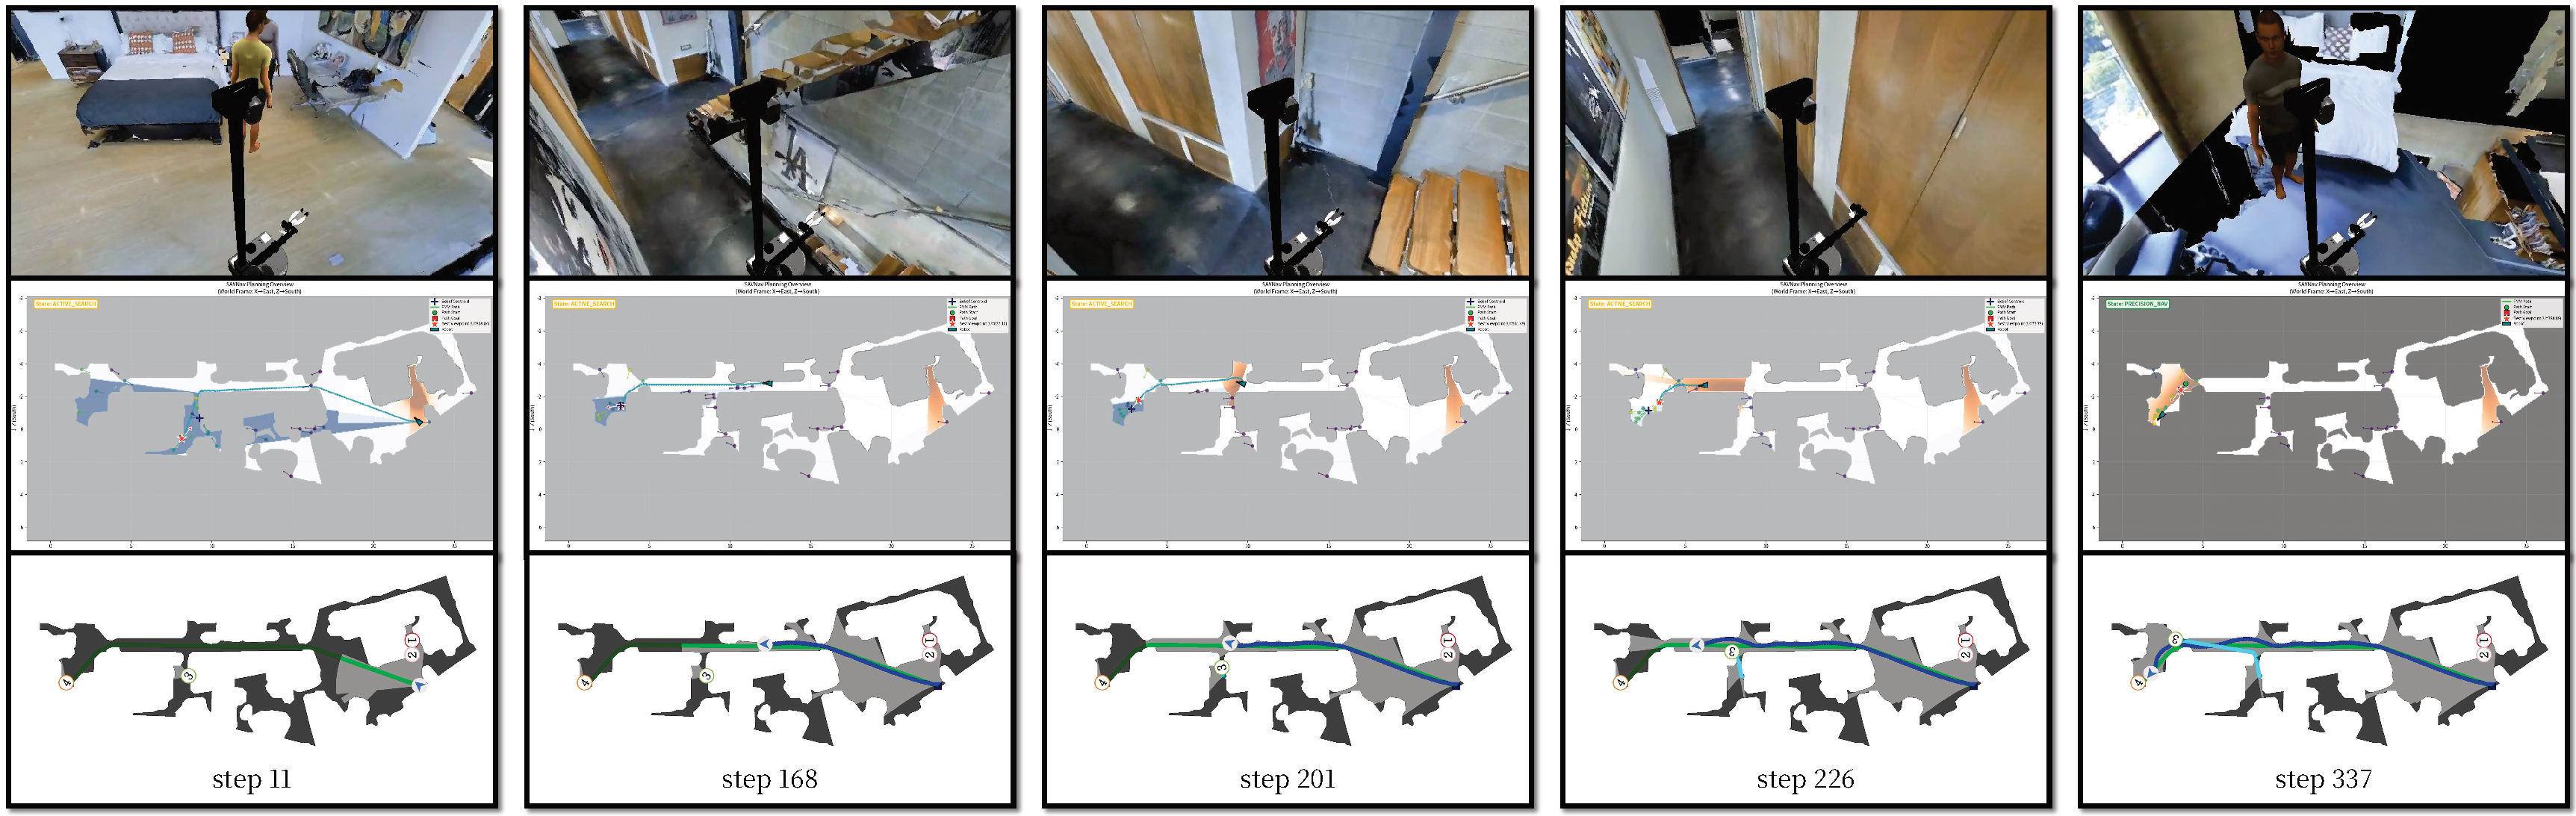
\includegraphics[width=1.00\linewidth]{figures/exp-q-sim.pdf}
	\caption{Qualitative navigation trajectories across the three scenarios. (a) In the crowded social scenario, SAVNav proactively routes around a SCG. (b) In the hidden boundary scenario, SAVNav anticipates NLOS footsteps and yields at a blind corner, whereas vision-only and reactive baselines collide. (c) In the mixed home activity scenario, SAVNav balances target search with dynamic yielding.}
	\label{fig:qualitative_results}
\end{figure*}

Fig.~\ref{fig:qualitative_results} illustrates representative trajectories generated by SAVNav compared to the baselines. In the crowded social scenario, SAVNav generates a smooth, socially compliant path that respects the static interaction zone of the SCG, whereas socially-unaware AVNav interrupts the group. In the hidden boundary scenario, the topology-aware acoustic anticipation allows SAVNav to execute a wide, defensive turn around a blind corner, safely avoiding an approaching DP before establishing LOS. In contrast, Falcon approaches the corner tightly, leading to an NLOS collision.

\subsection{Real-World Experiments}
\label{subsec:exp-realworld}

% TODO: Hardware setup, scenarios, and sim-to-real transfer results.

